\documentclass[english]{article}

\usepackage{babel}
\usepackage{graphicx}
\usepackage{alltt}
\usepackage{url}
\usepackage{tabularx}
%\usepackage{ngerman}
\usepackage{longtable}
\usepackage{color}
\usepackage{framed}

\usepackage{xifthen}
\newboolean{showbackdoors}
\setboolean{showbackdoors}{true}  % set to false to hide subsection on backdoors for reviewing group


\newenvironment{prettytablex}[1]{\vspace{0.3cm}\noindent\tabularx{\linewidth}{@{\hspace{\parindent}}#1@{}}}{\endtabularx\vspace{0.3cm}}
%\newenvironment{prettytable}{\prettytablex{l X}}{\endprettytablex}



\title{\huge\sffamily\bfseries System Description and Risk Analysis}
\author{B\"ahler Alessio \and Enz Andreas \and Niederberger Matthias}
\date{\today}


\begin{document}
\maketitle

%% **** please observe the page limit **** 
%% (it is not allowed to change the font size or page geometry to gain more space)
%% comment or remove lines below before hand-in

%%%%%%%%%%%%%%%%%%%%%%%%%%%%%%%%%%%%%%%%%%%%%%

\tableofcontents
\pagebreak


\section{System Characterization}

\subsection{System Overview}


%%% Describe the system's mission,  the system boundaries,
%%% and the overall system architecture, including the main subsystems and
%%% their relationships.   This description should provide a high-level
%%% overview of the system, e.g., suitable for managers, that complements
%%% the more technical description that follows.

\centerline{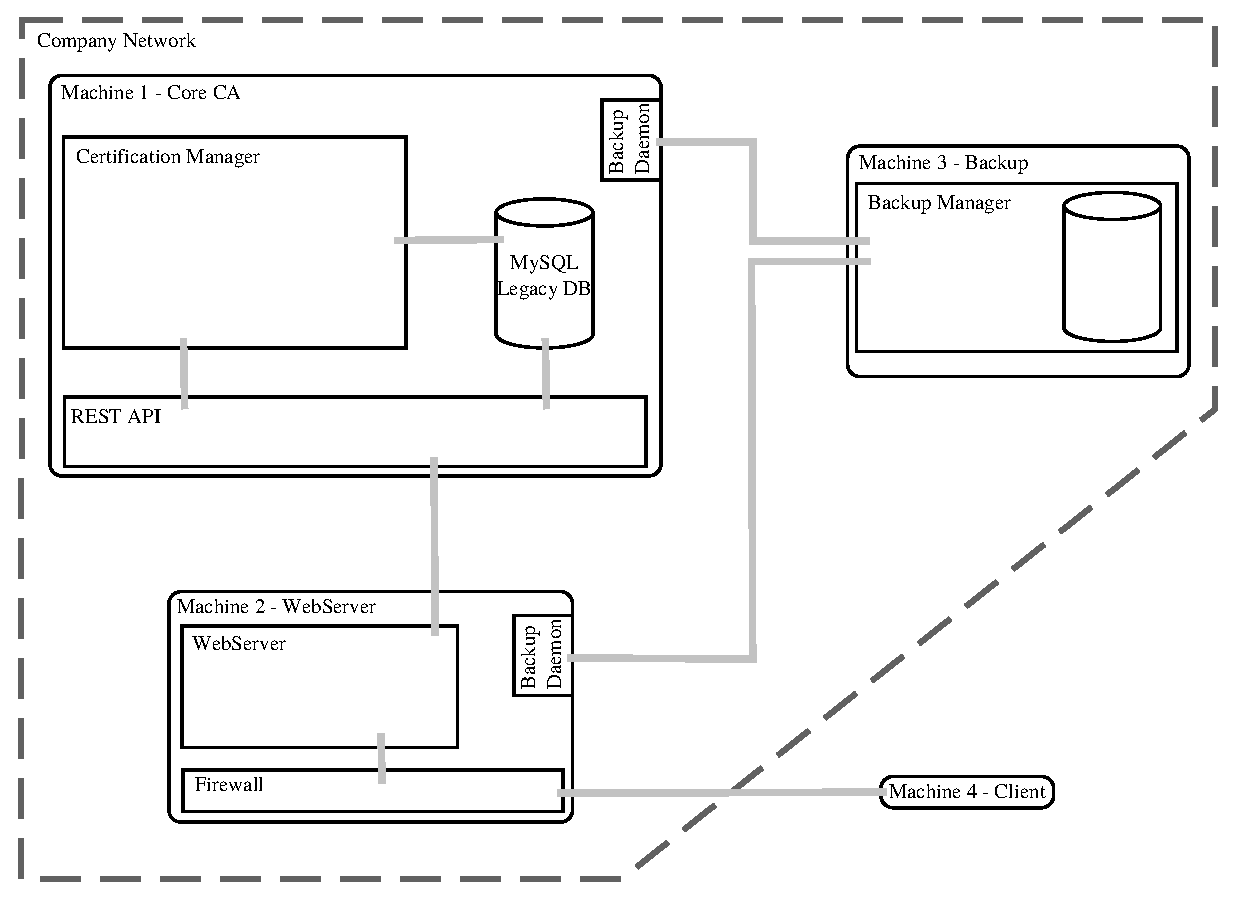
\includegraphics[width=1\textwidth]{res/system_arch.eps}}


\subsection{Components}

%%% List all system components and their interfaces, subdivided, for example, into
%%%   categories such as platforms, applications, data records, etc. For
%%%   each component, state its relevant properties.



\section{Risk Analysis and Security Measures}

\subsection{Assets}

TODO: Describe the relevant assets and their required security
  properties. For example, data objects, access restrictions,
  configurations, etc.
 
\textbf{Physical Assets}
\begin{itemize}
\item Web Server Machine
\item Core CA Machine
\item Backup Machine
\end{itemize}

\textbf{Logical Assets}
\begin{itemize}
\item Software
\item Certificates
\item Keys
\item User data
\item Configuration files
\item Logs
\end{itemize}

\textbf{Persons}
\begin{itemize}
\item System Administrator
\item CA Administrator
\item Users (Employees and Informants)
\end{itemize}

\textbf{Intangible Goods}
\begin{itemize}
\item Company Reputation
\end{itemize}

\subsection{Threat Sources}

TODO: Name and describe potential threat sources (\emph{not} threats!) including their motivation.

\begin{itemize}
\item Nature: probably not relevant since it targets availability
\item Users: Employees (includes also cleaning personnel etc.) and Informants can act maliciously or be careless/poorly trained
\item Competitors: may be interested in obtaining confidential information to gain an advantage, blackmail or cause harm by publishing it. May resort to Skilled Hackers to achieve their goals.
\item "Victims": subjects of investigative reports that were publicly exposed and may want to get revenge by causing any kind of damage. May resort to Skilled Hackers to achieve their goals.
\item Organized Crime: can directly or indirectly be "Victim", could be interested in blackmailing the Company to gain money or just to obtain important information that can be sold on the black market/used for other illegal activities.
\item Malware: TODO
\item Expert Hackers: A skilled hacker has expert knowledge for some systems. He can write his own code and may use unknown or unpublished vulnerabilities (from book). May itself be a "Victim" or act for monetary interests.
\item Script Kiddies: This type of adversary has basic computer knowledge and uses mainly known vulnerabilities for which exploits are available on the Internet. However, he might write scripts to automate tasks or use tools to automatically create malware. His main motivations are challenge, glory and destruction (from book).
\item Organizatorial Deficiencies (from SecEng slides): lack in employee training, poor/non-existing/non-enforced security measures (E.g. TODO) can weaken the overall security of the system.
\item Hardware Failures (from SecEng slides): TODO
\end{itemize}

\subsection{Risks Definitions}

Define likelihood, impact and risk level using the following three
  tables. TODO: source from book.

%\subsubsection{Tools}

\begin{center}
\begin{tabular}{|l|p{0.8\textwidth}|}
\hline
%\multicolumn{2}{|c|}{\bf Likelihood} \\
%\hline
Likelihood & Description \\
\hline
\hline
High   & The threat source is highly motivated and sufficiently capable of exploiting a given vulnerability in order to change the asset?s state. The controls to prevent the vulnerability from being exploited are ineffective. \\
\hline
Medium & The threat source is motivated and capable of exploiting a given vulnerability in order to change the asset?s state, but controls are in place that may impede a successful exploit of the vulnerability. \\
\hline
Low   & The threat source lacks motivation or capabilities to exploit a given vulnerability in order to change the asset?s state. Another possibility that results in a low likelihood is the case where controls are in place that prevent (or at least significantly impede) the vulnerability from being exercised. \\
\hline
\end{tabular}
\hspace{3em}
\begin{tabular}{|l|p{0.8\textwidth}|}
\hline
\multicolumn{2}{|c|}{\bf Impact} \\
\hline
Impact & Description \\
\hline
\hline
High   & The event (1) may result in a highly costly loss of major tangible assets or resources; (2) may significantly violate, harm, or impede an organization?s mission, reputation, or interest; or (3) may result in human death or serious injury. \\
\hline
Medium & The event (1) may result in a costly loss of tangible assets or resources; (2) may violate, harm, or impede an organization?s mission, reputation, or interest, or (3) may result in human injury. \\
\hline
Low   & The event (1) may result in a loss of some tangible assets or resources or (2) may noticeably affect an organization?s mission, reputation, or inter- est. \\
\hline
\end{tabular}
\end{center}

\vspace{5mm}

\begin{center}
\begin{tabular}{|l|c|c|c|}
\hline
\multicolumn{4}{|c|}{{\bf Risk Level}} \\
\hline
{{\bf Likelihood}} & \multicolumn{3}{c|}{{\bf Impact}} \\ %\cline{2-4}
     & Low & Medium & High \\  \hline
 High & Low & Medium & High  \\
\hline
 Medium & Low & Medium & Medium \\
\hline
 Low & Low & Low & Low \\
\hline
\end{tabular}
\end{center}


\subsection{Risk Evaluation}

List all potential threats and the corresponding countermeasures. Estimate the risk based on the information about the threat, the threat sources and the corresponding countermeasure. Adhere to the risk definitions you have given above. As a sanity check, there should be at least one high-risk entry.


\subsubsection{{\it Evaluation Asset X}}

Evaluate the likelihood, impact and the resulting risk,  \emph{after implementation of the corresponding countermeasures}. Formulate the threats in active, not passive, 
voice: who (threat source) does what (threat action)? 

\begin{footnotesize}
\begin{prettytablex}{llp{5.5cm}lll}
No. & Threat &  Countermeasure(s) & L & I & Risk \\
\hline
1 & ... & ... & {\it Low} & {\it Low} & {\it Low} \\
\hline
2 & ... & ...& {\it Medium} & {\it High} & {\it Medium} \\
\hline
\end{prettytablex}
\end{footnotesize}



\subsubsection{{\it Evaluation Asset y}}

\begin{footnotesize}
\begin{prettytablex}{llp{5.5cm}lll}
No. & Threat & Countermeasure(s) & L & I & Risk \\
\hline
1 & ... & ... & {\it Low} & {\it Low} & {\it Low} \\
\hline
2 & ... & ...& {\it Medium} & {\it High} & {\it Medium} \\
\hline
\end{prettytablex}
\end{footnotesize}

\subsubsection{Detailed Description of Selected Countermeasures}

Optionally explain the details of the countermeasures mentioned above.



\subsubsection{Risk Acceptance}

List all medium and high risks, according to the evaluation above. For each risk, propose additional countermeasures that could be implemented to further reduce the risks.

\begin{footnotesize}
\begin{prettytablex}{p{2cm}X}
No. of threat & Proposed additional countermeasure including expected impact  \\
\hline
... & ... \\
\hline
... & ... \\
\hline
\end{prettytablex}
\end{footnotesize}

\end{document}

%%% Local Variables: 
%%% mode: latex
%%% TeX-master: "../../book"
%%% End: 
